\chapter{Background} \label{chap:sota}

\section*{}

\section{Introduction}

- explain gene expression

- explain importance and applications of gene expression profilling

- explain that nowadays sequencing data is easier and cheaper to obtain, but
  harder to process

- explain that there are several techniques to obtain gene expression
  information

- explain that in the thesis only RNA-Seq will be analysed

\begin{figure}[t]
  \begin{center}
    \leavevmode
    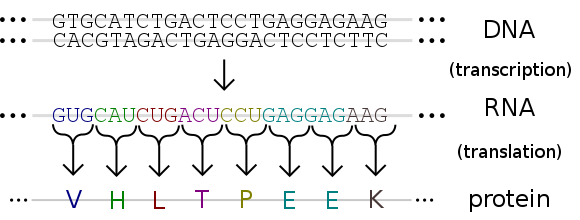
\includegraphics[width=0.6\textwidth]{gene_expr}
    \caption{Representation of the gene expression process \cite{madprime2006}}
    \label{fig:arch}
  \end{center}
\end{figure}

\section{Genome Assembly and \rnaseq}\label{sec:assembly}

\subsection{Assembly Methods}\label{sec:seqtools}

\subsection{\rnaseq{} Tools}\label{sec:seqtools}

\subsection{Common Data Formats}\label{sec:formats}

\section{Machine Learning}\label{sec:mlearning}

\section{Conclusions}
